
\section{Системийн загвар}

\subsection{Системийн архитектур}
Системийн үндсэн архитектур нь 3 шатлалт аргыг ашиглан хөгжүүлсэн. Хэрэглэгч талаас веб хөтөч ашиглан HTTP хүсэлт илгээнэ. 
Сервер талаас өгөгдлийн санг ашиглан API бэлдэн хэрэглэгчрүү  HTTP хүсэлтийн хариу өгөх зарчимаар ажиллана.
\begin{figure}[h]
    \centering
    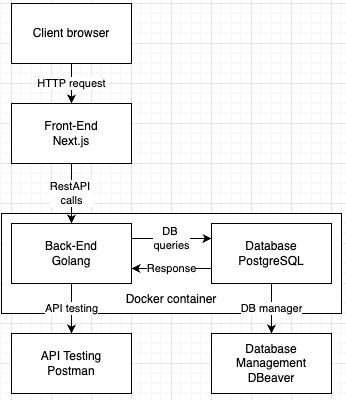
\includegraphics[scale=0.8]{src/images/diagram/arch.png}
    \caption{Системийн архитектурын диаграмм}
    \label{fig:system_architecture_diagram}
\end{figure}

\subsection{Системийн зохиомж}

\subsubsection{Системийн ажлын явцын диаграмм}
Энэхүү диаграммд админ, менежер, ажилтан гэсэн гурван төрлийн оролцогч
(тоглогч) бий. Диаграмм нь оролцогчдын хийж болох үйлдлүүдийг болон тэдгээрийн
хоорондын харилцаа, холбоог харуулж байна. Үйлчлүүлэгч, админ, ажилтан тус бүр нь
өөрийн хариуцсан үйлдлүүдийг гүйцэтгэх бөгөөд тэдгээрийн харилцан үйлчлэл, эрхийн
түвшин, үүрэг хариуцлагын хил хязгаарыг диаграммаас ойлгомжтой байдлаар харах
боломжтой.
\begin{figure}[h]
    \centering
    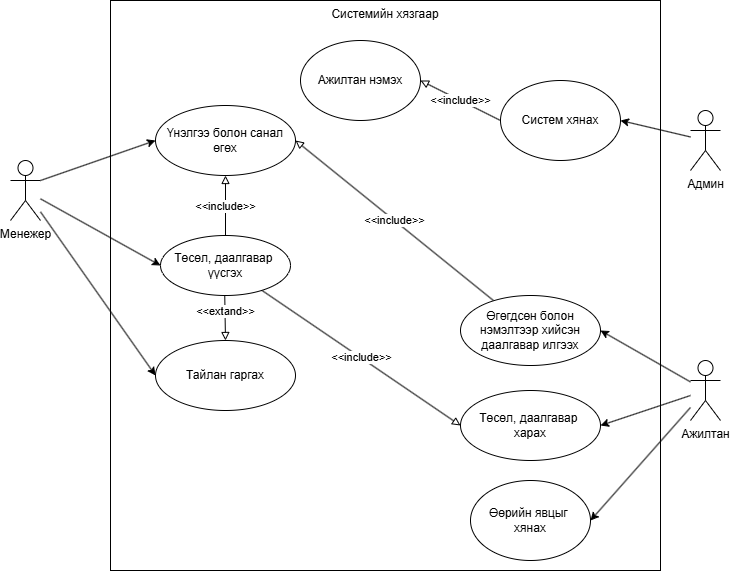
\includegraphics[scale=0.6]{src/images/diagram/usecase.png}
    \caption{Системийн ажлын явцын диаграмм}
    \label{fig:system_usecase_diagram}
\end{figure}

\subsubsection{Системийн нэгж хоорондын харилцаа хамаарлын диаграмм}
Уг диаграмм нь системийн өгөгдөл бүрдүүлэх бүх гол мэдээллүүдийн ерөнхий
бүтцийг харуулж байна. Системийг цаашид хөгжүүлэх үед уян хатан, өргөтгөх боломжтой
байдлаар диаграммыг боловсруулсан. Объектуудын хоорондын харилцаа, тэдгээрийн
холбоосууд нь системийг нэмэлт функц, боломжуудаар өргөжүүлэхэд хялбар, логик
уялдаатай байлгах зорилготой. Энэ нь системийг илүү үр ашигтай удирдах, өгөгдлийг
найдвартай зохицуулах үндсэн суурь болж өгнө.
\begin{figure}[H]
    \centering
    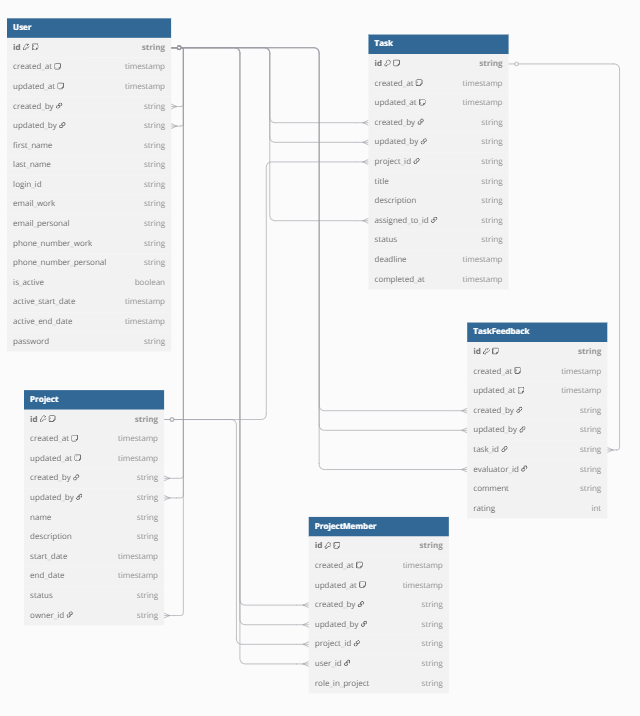
\includegraphics[scale=0.8]{src/images/diagram/projectTaskErd.png}
    \caption{Төсөл болон даалгаврын харилцан хамаарлын диаграмм}
    \label{fig:project_task_erd}
\end{figure}
\begin{figure}[H]
    \centering
    \includegraphics[scale=0.8]{src/images/diagram/employeeErd.png}
    \caption{Ажилтны нэгж хоорондын харилцан хамаарлын диаграмм}
    \label{fig:employee_erd}
\end{figure}
\begin{figure}[H]
    \centering
    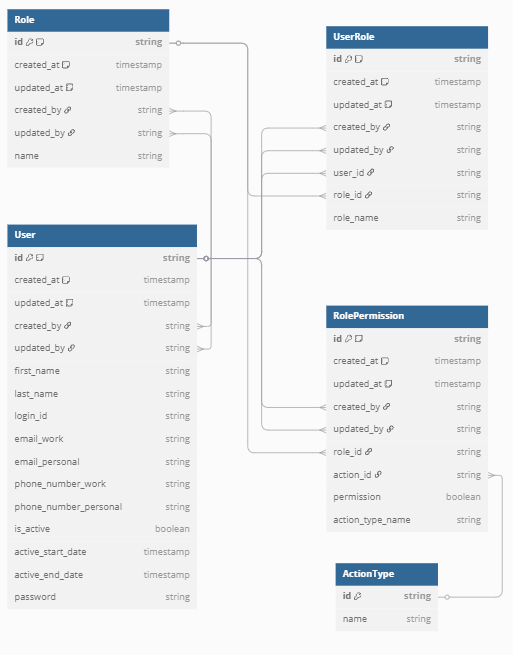
\includegraphics[scale=0.8]{src/images/diagram/userRoleErd.png}
    \caption{Ажилтан болон түүний эрхийн харилцан хамаарлын диаграмм}
    \label{fig:user_role_erd}
\end{figure}

\subsubsection{Дарааллын диаграмм}
Дарааллын диаграмм нь системийн бүрэлдэхүүн хэсгүүдийн хоорондын харилцан үйлчлэлийг цаг 
хугацааны дарааллаар харуулдаг UML-ийн нэг төрлийн диаграмм юм. Энэ нь тодорхой үйлдэл, жишээ 
нь даалгаврын илгээлт гэх мэт процессын явцад объектуудын хоорондох мессежийн урсгалыг тодорхойлдог.

\begin{figure}[H]
    \centering
    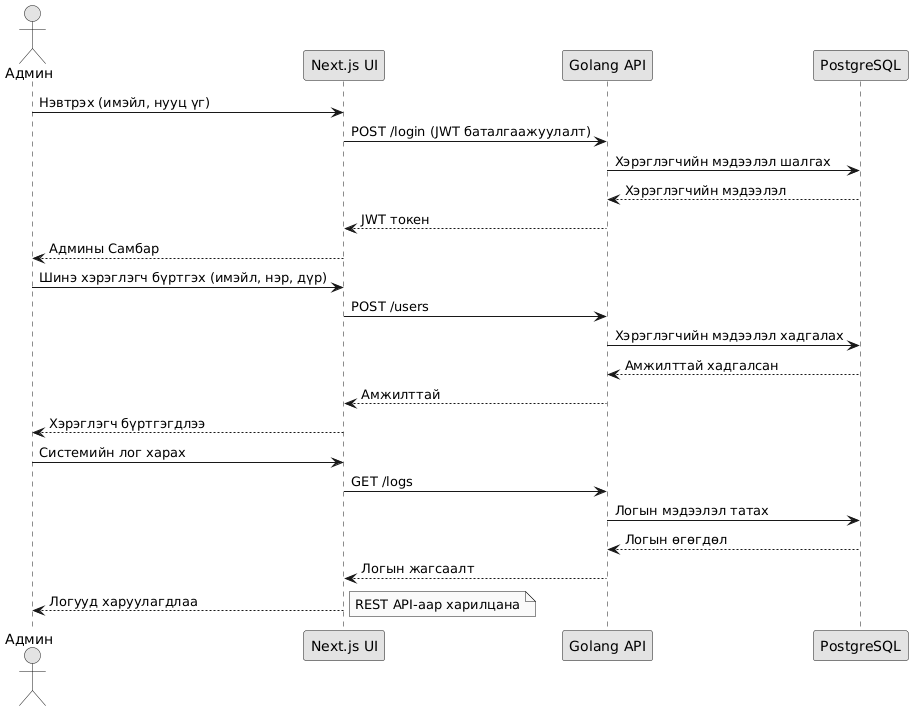
\includegraphics[scale=0.5]{src/images/diagram/admin-seq.png}
    \caption{Админ дарааллын диаграмм}
    \label{fig:admin_seq}
\end{figure}
\begin{figure}[H]
    \centering
    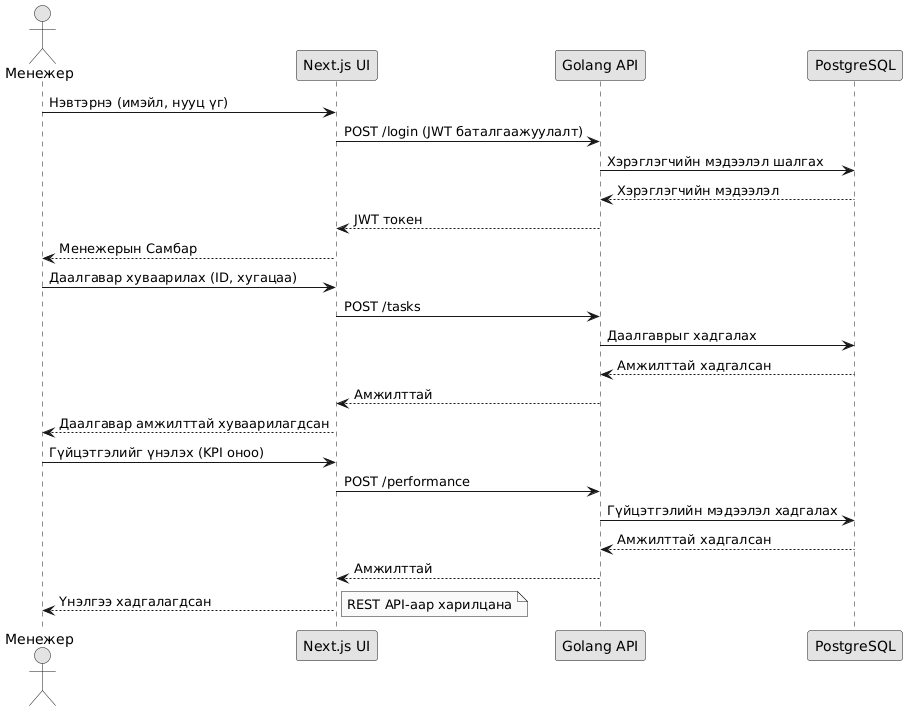
\includegraphics[scale=0.5]{src/images/diagram/manager_seq.png}
    \caption{Менежер дарааллын диаграмм}
    \label{fig:employee_seq}
\end{figure}
\begin{figure}[H]
    \centering
    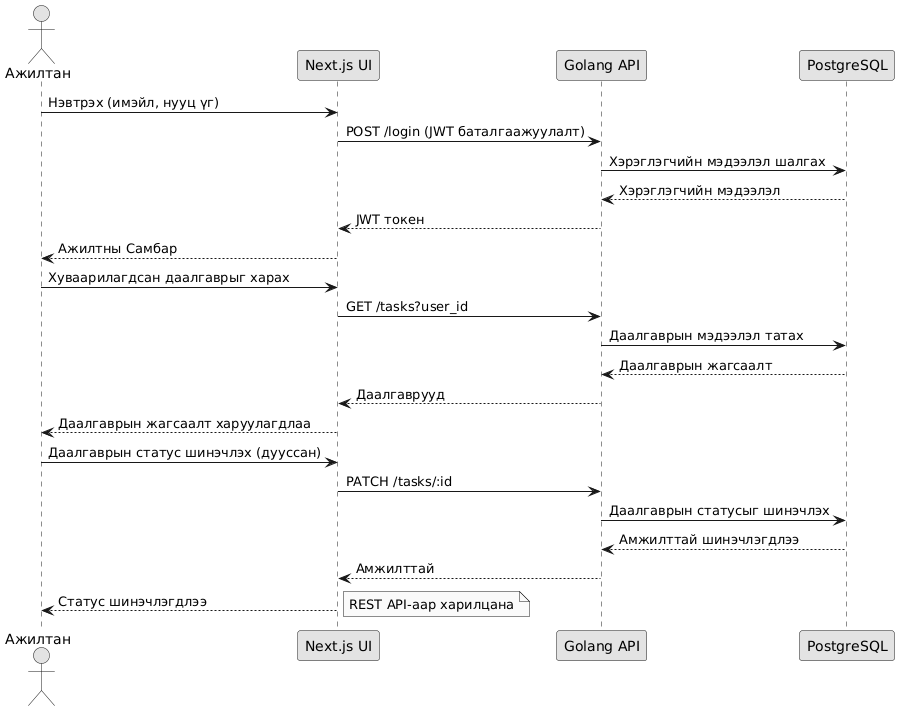
\includegraphics[scale=0.5]{src/images/diagram/employee_seq.png}
    \caption{Ажилтан дарааллын диаграмм}
    \label{fig:emp_seq}
\end{figure}